\documentclass[]{article}
\usepackage{lmodern}
\usepackage{amssymb,amsmath}
\usepackage{ifxetex,ifluatex}
\usepackage{fixltx2e} % provides \textsubscript
\ifnum 0\ifxetex 1\fi\ifluatex 1\fi=0 % if pdftex
  \usepackage[T1]{fontenc}
  \usepackage[utf8]{inputenc}
\else % if luatex or xelatex
  \ifxetex
    \usepackage{mathspec}
  \else
    \usepackage{fontspec}
  \fi
  \defaultfontfeatures{Ligatures=TeX,Scale=MatchLowercase}
\fi
% use upquote if available, for straight quotes in verbatim environments
\IfFileExists{upquote.sty}{\usepackage{upquote}}{}
% use microtype if available
\IfFileExists{microtype.sty}{%
\usepackage{microtype}
\UseMicrotypeSet[protrusion]{basicmath} % disable protrusion for tt fonts
}{}
\usepackage[margin=1in]{geometry}
\usepackage{hyperref}
\hypersetup{unicode=true,
            pdftitle={MVA Final Project},
            pdfauthor={Javier Ferrando Monsonis; Marcel Porta Valles; Mehmet Fatih ??agil},
            pdfborder={0 0 0},
            breaklinks=true}
\urlstyle{same}  % don't use monospace font for urls
\usepackage{color}
\usepackage{fancyvrb}
\newcommand{\VerbBar}{|}
\newcommand{\VERB}{\Verb[commandchars=\\\{\}]}
\DefineVerbatimEnvironment{Highlighting}{Verbatim}{commandchars=\\\{\}}
% Add ',fontsize=\small' for more characters per line
\usepackage{framed}
\definecolor{shadecolor}{RGB}{248,248,248}
\newenvironment{Shaded}{\begin{snugshade}}{\end{snugshade}}
\newcommand{\KeywordTok}[1]{\textcolor[rgb]{0.13,0.29,0.53}{\textbf{#1}}}
\newcommand{\DataTypeTok}[1]{\textcolor[rgb]{0.13,0.29,0.53}{#1}}
\newcommand{\DecValTok}[1]{\textcolor[rgb]{0.00,0.00,0.81}{#1}}
\newcommand{\BaseNTok}[1]{\textcolor[rgb]{0.00,0.00,0.81}{#1}}
\newcommand{\FloatTok}[1]{\textcolor[rgb]{0.00,0.00,0.81}{#1}}
\newcommand{\ConstantTok}[1]{\textcolor[rgb]{0.00,0.00,0.00}{#1}}
\newcommand{\CharTok}[1]{\textcolor[rgb]{0.31,0.60,0.02}{#1}}
\newcommand{\SpecialCharTok}[1]{\textcolor[rgb]{0.00,0.00,0.00}{#1}}
\newcommand{\StringTok}[1]{\textcolor[rgb]{0.31,0.60,0.02}{#1}}
\newcommand{\VerbatimStringTok}[1]{\textcolor[rgb]{0.31,0.60,0.02}{#1}}
\newcommand{\SpecialStringTok}[1]{\textcolor[rgb]{0.31,0.60,0.02}{#1}}
\newcommand{\ImportTok}[1]{#1}
\newcommand{\CommentTok}[1]{\textcolor[rgb]{0.56,0.35,0.01}{\textit{#1}}}
\newcommand{\DocumentationTok}[1]{\textcolor[rgb]{0.56,0.35,0.01}{\textbf{\textit{#1}}}}
\newcommand{\AnnotationTok}[1]{\textcolor[rgb]{0.56,0.35,0.01}{\textbf{\textit{#1}}}}
\newcommand{\CommentVarTok}[1]{\textcolor[rgb]{0.56,0.35,0.01}{\textbf{\textit{#1}}}}
\newcommand{\OtherTok}[1]{\textcolor[rgb]{0.56,0.35,0.01}{#1}}
\newcommand{\FunctionTok}[1]{\textcolor[rgb]{0.00,0.00,0.00}{#1}}
\newcommand{\VariableTok}[1]{\textcolor[rgb]{0.00,0.00,0.00}{#1}}
\newcommand{\ControlFlowTok}[1]{\textcolor[rgb]{0.13,0.29,0.53}{\textbf{#1}}}
\newcommand{\OperatorTok}[1]{\textcolor[rgb]{0.81,0.36,0.00}{\textbf{#1}}}
\newcommand{\BuiltInTok}[1]{#1}
\newcommand{\ExtensionTok}[1]{#1}
\newcommand{\PreprocessorTok}[1]{\textcolor[rgb]{0.56,0.35,0.01}{\textit{#1}}}
\newcommand{\AttributeTok}[1]{\textcolor[rgb]{0.77,0.63,0.00}{#1}}
\newcommand{\RegionMarkerTok}[1]{#1}
\newcommand{\InformationTok}[1]{\textcolor[rgb]{0.56,0.35,0.01}{\textbf{\textit{#1}}}}
\newcommand{\WarningTok}[1]{\textcolor[rgb]{0.56,0.35,0.01}{\textbf{\textit{#1}}}}
\newcommand{\AlertTok}[1]{\textcolor[rgb]{0.94,0.16,0.16}{#1}}
\newcommand{\ErrorTok}[1]{\textcolor[rgb]{0.64,0.00,0.00}{\textbf{#1}}}
\newcommand{\NormalTok}[1]{#1}
\usepackage{longtable,booktabs}
\usepackage{graphicx,grffile}
\makeatletter
\def\maxwidth{\ifdim\Gin@nat@width>\linewidth\linewidth\else\Gin@nat@width\fi}
\def\maxheight{\ifdim\Gin@nat@height>\textheight\textheight\else\Gin@nat@height\fi}
\makeatother
% Scale images if necessary, so that they will not overflow the page
% margins by default, and it is still possible to overwrite the defaults
% using explicit options in \includegraphics[width, height, ...]{}
\setkeys{Gin}{width=\maxwidth,height=\maxheight,keepaspectratio}
\IfFileExists{parskip.sty}{%
\usepackage{parskip}
}{% else
\setlength{\parindent}{0pt}
\setlength{\parskip}{6pt plus 2pt minus 1pt}
}
\setlength{\emergencystretch}{3em}  % prevent overfull lines
\providecommand{\tightlist}{%
  \setlength{\itemsep}{0pt}\setlength{\parskip}{0pt}}
\setcounter{secnumdepth}{0}
% Redefines (sub)paragraphs to behave more like sections
\ifx\paragraph\undefined\else
\let\oldparagraph\paragraph
\renewcommand{\paragraph}[1]{\oldparagraph{#1}\mbox{}}
\fi
\ifx\subparagraph\undefined\else
\let\oldsubparagraph\subparagraph
\renewcommand{\subparagraph}[1]{\oldsubparagraph{#1}\mbox{}}
\fi

%%% Use protect on footnotes to avoid problems with footnotes in titles
\let\rmarkdownfootnote\footnote%
\def\footnote{\protect\rmarkdownfootnote}

%%% Change title format to be more compact
\usepackage{titling}

% Create subtitle command for use in maketitle
\newcommand{\subtitle}[1]{
  \posttitle{
    \begin{center}\large#1\end{center}
    }
}

\setlength{\droptitle}{-2em}

  \title{MVA Final Project}
    \pretitle{\vspace{\droptitle}\centering\huge}
  \posttitle{\par}
    \author{Javier Ferrando Monsonis \\ Marcel Porta Valles \\ Mehmet Fatih ??agil}
    \preauthor{\centering\large\emph}
  \postauthor{\par}
      \predate{\centering\large\emph}
  \postdate{\par}
    \date{February 20, 2018}


\begin{document}
\maketitle

\begin{Shaded}
\begin{Highlighting}[]
\KeywordTok{library}\NormalTok{(magrittr)}
\KeywordTok{library}\NormalTok{(ggplot2)}
\KeywordTok{library}\NormalTok{(dplyr)}
\end{Highlighting}
\end{Shaded}

\begin{verbatim}
## 
## Attaching package: 'dplyr'
\end{verbatim}

\begin{verbatim}
## The following objects are masked from 'package:stats':
## 
##     filter, lag
\end{verbatim}

\begin{verbatim}
## The following objects are masked from 'package:base':
## 
##     intersect, setdiff, setequal, union
\end{verbatim}

\begin{Shaded}
\begin{Highlighting}[]
\KeywordTok{library}\NormalTok{(stringr)}
\KeywordTok{library}\NormalTok{(ggplot2)}

\KeywordTok{library}\NormalTok{(data.table)}
\end{Highlighting}
\end{Shaded}

\begin{verbatim}
## 
## Attaching package: 'data.table'
\end{verbatim}

\begin{verbatim}
## The following objects are masked from 'package:dplyr':
## 
##     between, first, last
\end{verbatim}

\begin{Shaded}
\begin{Highlighting}[]
\KeywordTok{library}\NormalTok{(dplyr)}
\KeywordTok{library}\NormalTok{(magrittr)}
\KeywordTok{library}\NormalTok{(ggplot2)}
\KeywordTok{library}\NormalTok{(gridExtra)}
\end{Highlighting}
\end{Shaded}

\begin{verbatim}
## 
## Attaching package: 'gridExtra'
\end{verbatim}

\begin{verbatim}
## The following object is masked from 'package:dplyr':
## 
##     combine
\end{verbatim}

\begin{Shaded}
\begin{Highlighting}[]
\KeywordTok{library}\NormalTok{(ggExtra)}
\KeywordTok{library}\NormalTok{(corrplot)}
\end{Highlighting}
\end{Shaded}

\begin{verbatim}
## corrplot 0.84 loaded
\end{verbatim}

\begin{Shaded}
\begin{Highlighting}[]
\KeywordTok{library}\NormalTok{(factoextra)}
\end{Highlighting}
\end{Shaded}

\begin{verbatim}
## Welcome! Related Books: `Practical Guide To Cluster Analysis in R` at https://goo.gl/13EFCZ
\end{verbatim}

\begin{Shaded}
\begin{Highlighting}[]
\KeywordTok{library}\NormalTok{(stringr)}
\KeywordTok{library}\NormalTok{(FactoMineR)}
\CommentTok{#library(kableExtra)}
\KeywordTok{library}\NormalTok{(knitr)}
\end{Highlighting}
\end{Shaded}

\begin{Shaded}
\begin{Highlighting}[]
\NormalTok{training_set <-}\StringTok{ }\NormalTok{train[,}\OperatorTok{-}\NormalTok{(}\DecValTok{1}\OperatorTok{:}\DecValTok{4}\NormalTok{)]}
\NormalTok{col_order <-}\StringTok{ }\KeywordTok{colnames}\NormalTok{(training_set)}

\NormalTok{test_set<-}\StringTok{ }\NormalTok{d_ss[,}\OperatorTok{-}\DecValTok{1}\NormalTok{][,}\OperatorTok{-}\NormalTok{(}\DecValTok{2}\OperatorTok{:}\DecValTok{4}\NormalTok{)]}
\KeywordTok{colnames}\NormalTok{(test_set)[}\DecValTok{1}\NormalTok{] <-}\StringTok{ "team1win"}
\NormalTok{test_set <-}\StringTok{ }\NormalTok{test_set[, col_order]}
\NormalTok{training_set}\OperatorTok{$}\NormalTok{elo_diff <-}\StringTok{ }\OtherTok{NULL}
\NormalTok{test_set}\OperatorTok{$}\NormalTok{elo_diff <-}\StringTok{ }\OtherTok{NULL}
\NormalTok{training_set}\OperatorTok{$}\NormalTok{diff_rank <-}\StringTok{ }\OtherTok{NULL}
\NormalTok{test_set}\OperatorTok{$}\NormalTok{diff_rank <-}\StringTok{ }\OtherTok{NULL}
\end{Highlighting}
\end{Shaded}

\begin{Shaded}
\begin{Highlighting}[]
\KeywordTok{kable}\NormalTok{(training_set[}\KeywordTok{sample}\NormalTok{(}\KeywordTok{nrow}\NormalTok{(train), }\DecValTok{6}\NormalTok{), ][,}\DecValTok{1}\OperatorTok{:}\DecValTok{10}\NormalTok{])}
\end{Highlighting}
\end{Shaded}

\begin{longtable}[]{@{}lrrrrrrrrrr@{}}
\toprule
& team1win & t1\_rank\_n & t2\_rank\_n & t1\_season\_elo &
t2\_season\_elo & elo\_prob\_1 & t1\_mpie & t2\_mpie & t1\_netrtg &
t2\_netrtg\tabularnewline
\midrule
\endhead
356 & 1 & 3 & 6 & 1856.137 & 1887.825 & 0.4545238 & 0.6262022 &
0.6137100 & 17.895837 & 23.247435\tabularnewline
685 & 0 & 6 & 3 & 1801.625 & 1926.582 & 0.3275457 & 0.5565142 &
0.5550160 & 12.281486 & 2.793131\tabularnewline
245 & 0 & 3 & 2 & 1959.413 & 1885.683 & 0.6045406 & 0.5616776 &
0.6209522 & 7.674065 & 20.702310\tabularnewline
419 & 1 & 2 & 7 & 2041.983 & 1914.979 & 0.6750457 & 0.6355244 &
0.5715324 & 25.295345 & 5.442056\tabularnewline
290 & 0 & 4 & 5 & 1879.756 & 1726.106 & 0.7077496 & 0.6142832 &
0.6469077 & 16.819462 & 35.533848\tabularnewline
454 & 1 & 2 & 15 & 1894.235 & 1575.011 & 0.8626647 & 0.6026319 &
0.5514985 & 18.796633 & 5.907027\tabularnewline
\bottomrule
\end{longtable}

\begin{Shaded}
\begin{Highlighting}[]
\CommentTok{#Train model with train data}
\CommentTok{#Add predictions to dss}
\CommentTok{#Merge d_ss with test_outcome_tournament (games that occurred) -> validation}
\CommentTok{#validation has target and Pred for every game that occurered 2014-2018}
\CommentTok{#Apply LogLoss to validation$Pred and validation$team1win}


\CommentTok{# #logistic regression model: differences}
\CommentTok{# model <- glm(team1win ~ }
\CommentTok{#                diff_rank +}
\CommentTok{#                t1_rank_n +}
\CommentTok{#                #t2_rank_n +}
\CommentTok{#                t1_season_elo +}
\CommentTok{#                t2_season_elo +}
\CommentTok{#                #elo_prob_1 +}
\CommentTok{#                t1_mpie +}
\CommentTok{#                t2_mpie +}
\CommentTok{#                t1_netrtg +}
\CommentTok{#                t2_netrtg}
\CommentTok{#              ,}
\CommentTok{#              }
\CommentTok{#              data = training_set, family = binomial)}

\NormalTok{model <-}\StringTok{ }\KeywordTok{glm}\NormalTok{(team1win }\OperatorTok{~}\StringTok{ }\NormalTok{.}
\NormalTok{             ,}
             
             \DataTypeTok{data =}\NormalTok{ training_set, }\DataTypeTok{family =}\NormalTok{ binomial)}


\CommentTok{#Predict on every possible matchup}
\NormalTok{predict <-}\StringTok{ }\KeywordTok{data.frame}\NormalTok{(}\DataTypeTok{Pred =} \KeywordTok{predict}\NormalTok{(model, }\DataTypeTok{newdata =}\NormalTok{ test_set, }\DataTypeTok{type =} \StringTok{'response'}\NormalTok{))}
\NormalTok{d_ss <-}\StringTok{ }\NormalTok{d_ss }\OperatorTok\StringTok{ }\KeywordTok{mutate}\NormalTok{(}\DataTypeTok{Pred =}\NormalTok{ predict}\OperatorTok{$}\NormalTok{Pred)}\CommentTok{# %>% dplyr::select(ID, Pred) Change sample submission pred=0.5 to model predicition}

\NormalTok{d_ss_fin <-}\StringTok{ }\NormalTok{sample_submission }\OperatorTok\StringTok{ }\KeywordTok{mutate}\NormalTok{(}\DataTypeTok{Pred =}\NormalTok{ d_ss}\OperatorTok{$}\NormalTok{Pred) }\CommentTok{#only matchup and prediction -> Results for kaggle}
\CommentTok{#write.csv(d_ss_fin, "submission_stage_2.csv", row.names = FALSE)}

\KeywordTok{summary}\NormalTok{(model)}
\end{Highlighting}
\end{Shaded}

\begin{verbatim}
## 
## Call:
## glm(formula = team1win ~ ., family = binomial, data = training_set)
## 
## Deviance Residuals: 
##     Min       1Q   Median       3Q      Max  
## -2.3242  -0.8802   0.2700   0.8947   2.5987  
## 
## Coefficients:
##                Estimate Std. Error z value Pr(>|z|)   
## (Intercept)   -7.206253   4.727048  -1.524  0.12739   
## t1_rank_n     -0.089333   0.039574  -2.257  0.02398 * 
## t2_rank_n      0.112791   0.041428   2.723  0.00648 **
## t1_season_elo  0.003624   0.003197   1.133  0.25708   
## t2_season_elo -0.002286   0.003169  -0.721  0.47082   
## elo_prob_1    -0.774010   2.608352  -0.297  0.76666   
## t1_mpie        6.509649   4.661552   1.396  0.16258   
## t2_mpie        2.520763   4.635233   0.544  0.58656   
## t1_netrtg      0.001556   0.018493   0.084  0.93293   
## t2_netrtg     -0.021832   0.018828  -1.160  0.24624   
## ---
## Signif. codes:  0 '***' 0.001 '**' 0.01 '*' 0.05 '.' 0.1 ' ' 1
## 
## (Dispersion parameter for binomial family taken to be 1)
## 
##     Null deviance: 988.02  on 712  degrees of freedom
## Residual deviance: 764.18  on 703  degrees of freedom
## AIC: 784.18
## 
## Number of Fisher Scoring iterations: 5
\end{verbatim}

\begin{Shaded}
\begin{Highlighting}[]
\KeywordTok{kable}\NormalTok{(}\KeywordTok{summary}\NormalTok{(model)}\OperatorTok{$}\NormalTok{coefficients)}
\end{Highlighting}
\end{Shaded}

\begin{longtable}[]{@{}lrrrr@{}}
\toprule
& Estimate & Std. Error & z value &
Pr(\textgreater{}\textbar{}z\textbar{})\tabularnewline
\midrule
\endhead
(Intercept) & -7.2062527 & 4.7270477 & -1.5244722 &
0.1273908\tabularnewline
t1\_rank\_n & -0.0893334 & 0.0395736 & -2.2574005 &
0.0239831\tabularnewline
t2\_rank\_n & 0.1127913 & 0.0414276 & 2.7226099 &
0.0064768\tabularnewline
t1\_season\_elo & 0.0036236 & 0.0031973 & 1.1333294 &
0.2570760\tabularnewline
t2\_season\_elo & -0.0022855 & 0.0031693 & -0.7211487 &
0.4708180\tabularnewline
elo\_prob\_1 & -0.7740098 & 2.6083520 & -0.2967428 &
0.7666628\tabularnewline
t1\_mpie & 6.5096493 & 4.6615522 & 1.3964553 & 0.1625774\tabularnewline
t2\_mpie & 2.5207630 & 4.6352331 & 0.5438266 & 0.5865608\tabularnewline
t1\_netrtg & 0.0015563 & 0.0184935 & 0.0841542 &
0.9329338\tabularnewline
t2\_netrtg & -0.0218315 & 0.0188280 & -1.1595228 &
0.2462432\tabularnewline
\bottomrule
\end{longtable}

\begin{Shaded}
\begin{Highlighting}[]
\CommentTok{#Merge every possible matchup result predictions with real games and check test error}
\NormalTok{test_result <-}\StringTok{ }\KeywordTok{merge}\NormalTok{(}\DataTypeTok{x =}\NormalTok{ test_outcome_tournament, }\DataTypeTok{y =}\NormalTok{ d_ss[}\DecValTok{2}\OperatorTok{:}\DecValTok{5}\NormalTok{], }\DataTypeTok{by=}\KeywordTok{c}\NormalTok{(}\StringTok{"team1id"}\NormalTok{,}\StringTok{"team2id"}\NormalTok{,}\StringTok{"season"}\NormalTok{), }\DataTypeTok{all =} \OtherTok{FALSE}\NormalTok{)}

\KeywordTok{library}\NormalTok{(MLmetrics)}
\end{Highlighting}
\end{Shaded}

\begin{verbatim}
## 
## Attaching package: 'MLmetrics'
\end{verbatim}

\begin{verbatim}
## The following object is masked from 'package:base':
## 
##     Recall
\end{verbatim}

\begin{Shaded}
\begin{Highlighting}[]
\CommentTok{#library(forecast)}

\KeywordTok{LogLoss}\NormalTok{(}\DataTypeTok{y_pred =}\NormalTok{ test_result}\OperatorTok{$}\NormalTok{Pred, }\DataTypeTok{y_true =}\NormalTok{ test_result}\OperatorTok{$}\NormalTok{team1win)}
\end{Highlighting}
\end{Shaded}

\begin{verbatim}
## [1] 0.5589786
\end{verbatim}

\begin{Shaded}
\begin{Highlighting}[]
\NormalTok{pca_ncaa <-}\StringTok{ }\KeywordTok{PCA}\NormalTok{(training_set, }\DataTypeTok{quali.sup =} \DecValTok{1}\NormalTok{, }\DataTypeTok{scale.unit =} \OtherTok{TRUE}\NormalTok{,  }\DataTypeTok{graph =} \OtherTok{TRUE}\NormalTok{)}
\end{Highlighting}
\end{Shaded}

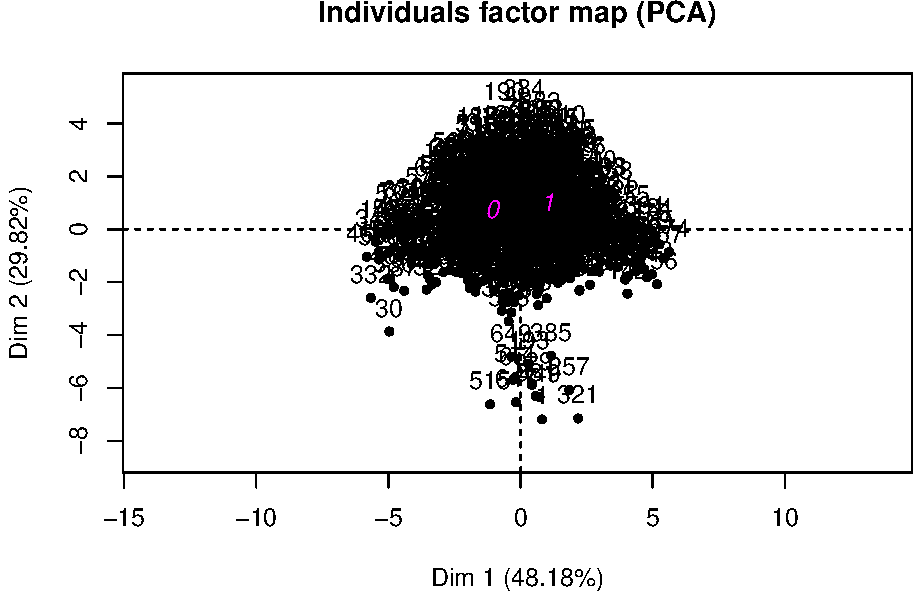
\includegraphics{data_prep_files/figure-latex/unnamed-chunk-5-1.pdf}
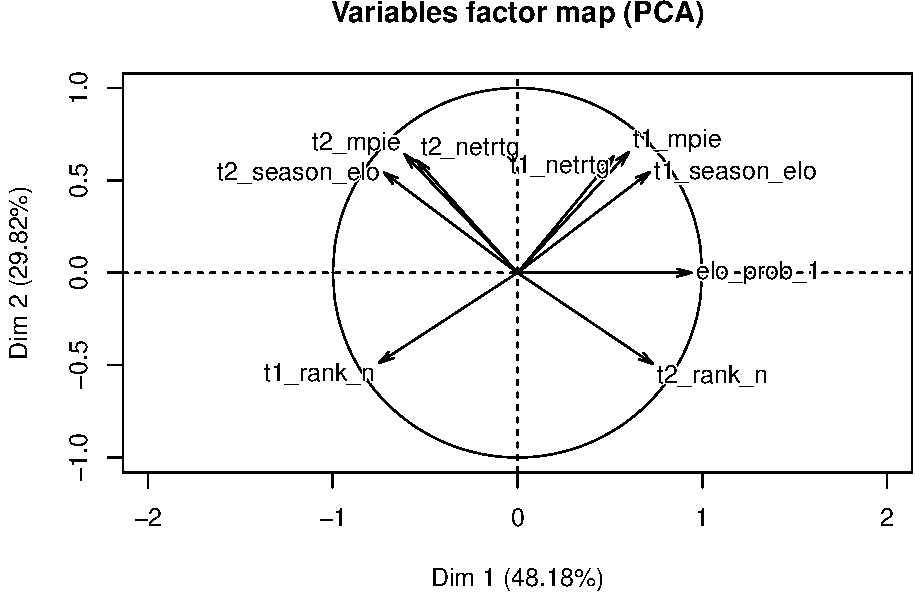
\includegraphics{data_prep_files/figure-latex/unnamed-chunk-5-2.pdf}

\begin{Shaded}
\begin{Highlighting}[]
\CommentTok{# #Regularized Logistic Regression}
\CommentTok{# #Total fail-> predictions wrong}
\CommentTok{# }
\CommentTok{# set.seed(123)}
\CommentTok{# library(glmnet)}
\CommentTok{# x <- model.matrix(team1win~., training_set)}
\CommentTok{# y <- training_set$team1win}
\CommentTok{# cv.lasso <- cv.glmnet(x, y , alpha = 1, family = "binomial")}
\CommentTok{# # Fit the final model on the training data}
\CommentTok{# model <- glmnet(x, y, alpha = 1, family = "binomial",}
\CommentTok{#                 lambda = cv.lasso$lambda.min)}
\CommentTok{# plot(cv.lasso)}
\CommentTok{# # Display regression coefficients}
\CommentTok{# coef(model)}
\CommentTok{# }
\CommentTok{# #### glmnet test}
\CommentTok{# }
\CommentTok{# x.test <- model.matrix(team1win~., test_set)}
\CommentTok{# }
\CommentTok{# probabilities <- model %>% predict(newx = x.test)}
\CommentTok{# ```}
\CommentTok{# }
\CommentTok{# ```\{r\}}
\CommentTok{# #Neural Network}
\CommentTok{# #Scale inputs}
\CommentTok{# library(nnet)}
\CommentTok{# library(caret)}
\CommentTok{# library(neuralnet)}
\CommentTok{# }
\CommentTok{# }
\CommentTok{# train_nnet_scaled <- as.data.frame(scale(training_set[-1]))}
\CommentTok{# train_nnet_scaled <- cbind(training_set$team1win,train_nnet_scaled)}
\CommentTok{# colnames(train_nnet_scaled)[1] <- "team1win"}
\CommentTok{# #train_nnet_scaled$team1win<- factor(train_nnet_scaled$team1win, labels=c(0,1))#not for neuralnet}
\CommentTok{# }
\CommentTok{# #nn1 <- nnet(team1win~t1_rank_n+t2_rank_n+elo_diff,data=train_nnet_scaled,entropy=T,size=100,decay=0,maxit=1000,trace=T)}
\CommentTok{# #predict <- data.frame(Pred = predict(nn1, newdata = d_ss_nnet_scaled))}
\CommentTok{# }
\CommentTok{# #10 fold cv trial}
\CommentTok{# }
\CommentTok{# ## We first split the available data into learning and test sets, selecting randomly 2/3 and 1/3 of the data}
\CommentTok{# ## We do this for a honest estimation of prediction performance}
\CommentTok{# }
\CommentTok{# names <- colnames(train_nnet_scaled)[-1] #choose the names you want}
\CommentTok{# a <- as.formula(paste('team1win ~ ' ,paste(names,collapse='+')))}
\CommentTok{# a}
\CommentTok{# #neuralnet DOESN'T need factors as target}
\CommentTok{# nn <- neuralnet(a, data=train_nnet_scaled, hidden=c(1), linear.output=FALSE, threshold=0.01)}
\CommentTok{# nn$result.matrix}
\CommentTok{# plot(nn)}
\CommentTok{# }
\CommentTok{# }
\CommentTok{# }
\CommentTok{# #nnet by means of train function, needs factors as target}
\CommentTok{# # model <- train(team1win~., data=train_nnet_scaled, method='nnet', maxit = 300,}
\CommentTok{# #                trControl=trainControl(method='cv'))}
\CommentTok{# test_set_scaled <- scale(test_set)}
\CommentTok{# }
\CommentTok{# #predict <- data.frame(Pred = predict (model, newdata=d_ss_nnet_scaled, type="prob"))}
\CommentTok{# }
\CommentTok{# test_set_scaled <- subset(test_set_scaled, select = colnames(test_set_scaled)[-1])}
\CommentTok{# nn.results <- compute(nn, test_set_scaled)}
\CommentTok{# }
\CommentTok{# #train in nnet prediction}
\CommentTok{# #d_ss <- d_ss %>% mutate(Pred = predict$Pred.1)# %>% dplyr::select(ID, Pred) Change sample submission pred=0.5 to model predicition}
\CommentTok{# }
\CommentTok{# #neuralnet prediction}
\CommentTok{# #d_ss$Pred <- NULL}
\CommentTok{# d_ss <- d_ss %>% mutate(Pred = as.numeric(nn.results$net.result))}
\CommentTok{# }
\CommentTok{# }
\CommentTok{# }
\CommentTok{# }
\CommentTok{# }
\CommentTok{# # d_ss_fin <- sample_submission %>% mutate(Pred = d_ss$Pred) #only matchup and prediction -> Results for kaggle}
\CommentTok{# # #write.csv(d_ss_fin, "submission_stage_2.csv", row.names = FALSE)}
\CommentTok{# # }
\CommentTok{# # }
\CommentTok{# # #############}
\CommentTok{# # set.seed(43)}
\CommentTok{# # N <- nrow(train_nnet_scaled)}
\CommentTok{# # learn <- sample(1:N, round(2*N/3))}
\CommentTok{# # (sizes <- 2*seq(1,10,by=2)) #different sizes}
\CommentTok{# # }
\CommentTok{# # ## specify 10x10 CV}
\CommentTok{# # trc <- trainControl (method="repeatedcv", number=10, repeats=10)}
\CommentTok{# # }
\CommentTok{# # model.10x10CV <- train (team1win ~., data = train_nnet_scaled, subset=learn, method='nnet', maxit = 500, trace = FALSE,tuneGrid = expand.grid(.size=sizes,.decay=0), trControl=trc)}
\CommentTok{# }
\CommentTok{# }
\CommentTok{# ```}
\CommentTok{# }
\CommentTok{# ```\{r\}}
\CommentTok{# #We can only test with 2014-2018 data}
\CommentTok{# #Merge every possible matchup result predictions with real games and check test error}
\CommentTok{# test_result <- merge(x = test_outcome_tournament, y = d_ss[2:5], by=c("team1id","team2id","season"), all = FALSE)}
\CommentTok{# }
\CommentTok{# library(MLmetrics)}
\CommentTok{# #library(forecast)}
\CommentTok{# }
\CommentTok{# LogLoss(y_pred = test_result$Pred, y_true = test_result$team1win)}
\CommentTok{# }
\CommentTok{# test_result$Pred<- factor(test_result$Pred, labels=c(0,1))#}
\CommentTok{# Accuracy(y_pred = test_result$Pred, y_true = test_result$team1win)}
\CommentTok{# }
\CommentTok{# ```}
\CommentTok{# }
\CommentTok{# ```\{r,echo=FALSE\}}
\CommentTok{# library(rpart)}
\CommentTok{# train_tree <- training_set}
\CommentTok{# train_tree$team1win<- factor(train_tree$team1win, labels=c(0,1))#not for neuralnet}
\CommentTok{# }
\CommentTok{# DecisionTree = rpart(team1win ~ ., data=train_tree,control=rpart.control(cp=0.001, xval=10),method='class')}
\CommentTok{# printcp(DecisionTree)}
\CommentTok{# }
\CommentTok{# treeSize = DecisionTree$cptable[,2]+1 #nsplit}
\CommentTok{# treeImpurity = DecisionTree$cptable[,3] #rel error}
\CommentTok{# cvImpurity = DecisionTree$cptable[,4] #xerror}
\CommentTok{# }
\CommentTok{# plot(treeSize, treeImpurity, main="R(T)", xlab="size of the tree", ylab="Relativity Impurity", type="o", col='red') }
\CommentTok{# lines(treeSize, cvImpurity ,type="o", col='blue')}
\CommentTok{# legend("topright", c("All training data","CV training data"), col=c('red', 'blue'), lty=1)}
\CommentTok{# ```}
\CommentTok{# }
\CommentTok{# ```\{r, echo=FALSE\}}
\CommentTok{# DecisionTree$cptable = as.data.frame(DecisionTree $cptable)}
\CommentTok{# ind = which.min(DecisionTree$cptable$xerror)}
\CommentTok{# xerr <-DecisionTree$cptable$xerror[ind]}
\CommentTok{# xstd <-DecisionTree$cptable$xstd[ind]}
\CommentTok{# }
\CommentTok{# i = 1}
\CommentTok{# while (DecisionTree$cptable$xerror[i] > xerr+xstd)\{}
\CommentTok{#   i = i+1}
\CommentTok{# \}}
\CommentTok{# #alfa = DecisionTree$cptable$CP[i]}
\CommentTok{# alfa = DecisionTree$cptable$CP[3]}
\CommentTok{# }
\CommentTok{# optimal <- prune(DecisionTree, cp=alfa)}
\CommentTok{# par(mfrow = c(1,1), xpd = NA)}
\CommentTok{# plot(optimal)}
\CommentTok{# text(optimal, use.n=T,cex=0.8,col="blue")}
\CommentTok{# }
\CommentTok{# #Tree prediction}
\CommentTok{# rpart_pred <- predict(DecisionTree,test_set,type='prob')[,1]}
\CommentTok{# rpart_pred_class <- predict(DecisionTree,test_set,type='class')}
\CommentTok{# d_ss <- d_ss %>% mutate(Pred = predict(DecisionTree,test_set,type='prob')[,1])}
\CommentTok{# #d_ss <- d_ss %>% mutate(Pred = predict(DecisionTree,test_set,type='class'))}
\CommentTok{# ```}
\CommentTok{# }
\CommentTok{# ```\{r, echo=FALSE\}}
\CommentTok{# library(randomForest)}
\CommentTok{# train_tree <- training_set}
\CommentTok{# train_tree$team1win<- factor(train_tree$team1win, labels=c(0,1))#not for neuralnet}
\CommentTok{# }
\CommentTok{# #Convert d_ss_tree$team1win to categorical values}
\CommentTok{# test_set_rf <- test_set}
\CommentTok{# test_set_rf$team1win <- NULL}
\CommentTok{# test_set_rf$team1win <- sample(c(0, 1), nrow(test_set_rf), replace=TRUE)}
\CommentTok{# }
\CommentTok{# test_set_rf <- test_set_rf[, col_order]}
\CommentTok{# test_set_rf$team1win<- factor(test_set_rf$team1win, labels=c(0,1))}
\CommentTok{# }
\CommentTok{# random_forest <- randomForest(formula = team1win ~.,}
\CommentTok{#                         data=train_tree,}
\CommentTok{#                         mtry=3,      # three predictor-vars selected randomly at each split}
\CommentTok{#                         xtest=test_set_rf[-1],}
\CommentTok{#                         ytest=test_set_rf$team1win,}
\CommentTok{#                         #ytest=as.factor(audit_imp$Adjusted[testRows]),}
\CommentTok{#                         importance=T,}
\CommentTok{#                         ntree=500,   # acceptably large value to ensure each sample row is predicted}
\CommentTok{#                                      # at least 2-digit nbr of times on average}
\CommentTok{#                         nodesize = 50,}
\CommentTok{#                         maxnodes = 40,}
\CommentTok{#                         norm.votes=T,}
\CommentTok{#                         keep.forest=TRUE)}
\CommentTok{# }
\CommentTok{# #rf_predictions_prob <- predict(random_forest, test_set_rf, type='prob')}
\CommentTok{# rf_predictions_class <- predict(random_forest, test_set_rf, type='class')}
\CommentTok{# #d_ss <- d_ss %>% mutate(Pred = rf_predictions_prob[,2])#For prob}
\CommentTok{# d_ss <- d_ss %>% mutate(Pred = rf_predictions_class)}
\CommentTok{# # }
\CommentTok{# # cf <- confusionMatrix(factor(df_rf_predictions), factor(rf_test$target), positive="1", dnn = c("Prediction", "True values"))}
\CommentTok{# # draw_confusion_matrix(cf)}
\CommentTok{# ```}
\CommentTok{# }
\CommentTok{# }
\CommentTok{# ```\{r, echo=FALSE\}}
\CommentTok{# library(caret)}
\CommentTok{# train_tree <- train[,-(1:4)]}
\CommentTok{# #train_tree$team1win<- factor(train_tree$team1win, labels=c(0,1))}
\CommentTok{# train_tree$team1win<- factor(train_tree$team1win, labels=c("win","loss"))#not for neuralnet}
\CommentTok{# }
\CommentTok{# # Example of Bagging algorithms}
\CommentTok{# control <- trainControl(method="repeatedcv", number=10, repeats=3)}
\CommentTok{# seed <- 7}
\CommentTok{# metric <- "logLoss"}
\CommentTok{# # Bagged CART}
\CommentTok{# set.seed(seed)}
\CommentTok{# fit.treebag <- train(team1win~., data=train_tree, method="treebag", metric=metric, trControl=control)}
\CommentTok{# # Random Forest}
\CommentTok{# set.seed(seed)}
\CommentTok{# fit.rf <- train(team1win~., data=train_tree, method="rf", metric=metric, trControl=control)}
\CommentTok{# # summarize results}
\CommentTok{# bagging_results <- resamples(list(treebag=fit.treebag, rf=fit.rf))}
\CommentTok{# summary(bagging_results)}
\CommentTok{# dotplot(bagging_results)}
\CommentTok{# ```}
\CommentTok{# }
\CommentTok{# ```\{r, echo=FALSE\}}
\CommentTok{# }
\CommentTok{# # Example of Stacking algorithms}
\CommentTok{# # create submodels}
\CommentTok{# train_ensemble <- training_set}
\CommentTok{# train_ensemble$diff_rank <- NULL}
\CommentTok{# train_ensemble$elo_diff <- NULL}
\CommentTok{# train_ensemble$team1win<- factor(train_ensemble$team1win, labels=c("win","loss"))#not for neuralnet}
\CommentTok{# }
\CommentTok{# library(caretEnsemble)}
\CommentTok{# control <- trainControl(method="repeatedcv", number=10, repeats=10, savePredictions='all', classProbs=TRUE,summaryFunction = mnLogLoss)}
\CommentTok{# algorithmList <- c('lda', 'glm', 'svmRadial')#knn disaster}
\CommentTok{# #algorithmList <- c('rpart', 'glm','svmRadial')}
\CommentTok{# set.seed(7)}
\CommentTok{# metric <- "logLoss"}
\CommentTok{# models <- caretList(team1win~., data=train_ensemble, trControl=control, methodList=algorithmList, metric=metric)}
\CommentTok{# }
\CommentTok{# }
\CommentTok{# }
\CommentTok{# greedy_ensemble <- caretEnsemble(}
\CommentTok{#   models, }
\CommentTok{#   metric="logLoss",}
\CommentTok{#   trControl=control)}
\CommentTok{# summary(greedy_ensemble)}
\CommentTok{# }
\CommentTok{# kable(modelCor(resamples(models)))}
\CommentTok{# }
\CommentTok{# summary(greedy_ensemble)}
\CommentTok{# results <- resamples(models)}
\CommentTok{# summary(results)}
\CommentTok{# dotplot(results)}
\CommentTok{# ensemble_pred <- predict(greedy_ensemble, newdata=test_set,type='prob')}
\CommentTok{# d_ss <- d_ss %>% mutate(Pred = ensemble_pred)#F}
\end{Highlighting}
\end{Shaded}


\end{document}
